\chapter{Brief explanation of FOC}
\section{FOC overview}
Field Oriented Control (FOC) is a closed loop control method for controlling torque of BLDC motors based on Clarke-Park Transformation.
Standard BLDC motor is aquipped with three stator windings, which are supplied with three phase currents.
To achive commutation and generate torque, propper voltage has to be provided to the stator windings by reading the phase currents ($i_a, i_b, i_c$).
Three phase currents reference frames can be decomposed into two orthogonal torque and flux reference frames using Clarke transformation, 
resulting in two currents ($i_\alpha$, $i_\beta$) in a stationary reference frame.

Park transformation is then applied to transform the currents from a stationary reference frame to a rotating reference frame, resulting in two DC currents ($i_d$, $i_q$), 
where $i_d$ is a flux current and $i_q$ is a torque current.

To control $i_d$ and $i_q$ currents, two independent proportional-integral (PI) controllers are used to update applied voltage to the stator windings based on the error between the reference and the measured currents.
In this implementation only the $i_q$ current reference is changed to control the torque, while the $i_d$ current reference is always set to zero to maximize the torque per ampere.

After getting new voltage references from the PI controllers, they need to be transformed back to three phase voltages using inverse Park and inverse Clarke transformations,
which can be then applied to the stator windings.

However applying the voltages directly from the inverse Park-Clarke transformations will achieve only aproximatelly 85 \% of the maximum voltage difference between the stator windings,
which is not optimal. \cite{svpwm_efficiency} To maximize the voltage difference between the stator windings, Space Vector Modulation (SVPWM) can be applied to the voltage references. 

Now that we can control the torque of the motor by controlling the $i_q$ current reference, a velocity control loop can be implemented on top of the torque control by 
using a PI controller to update the $i_q$ current reference based on the velocity error.

Aditionally, a position control loop can be implemented on top of the velocity control loop by using a PID controller to update the velocity reference based on the position error.

\begin{figure}[h]
    \centering
    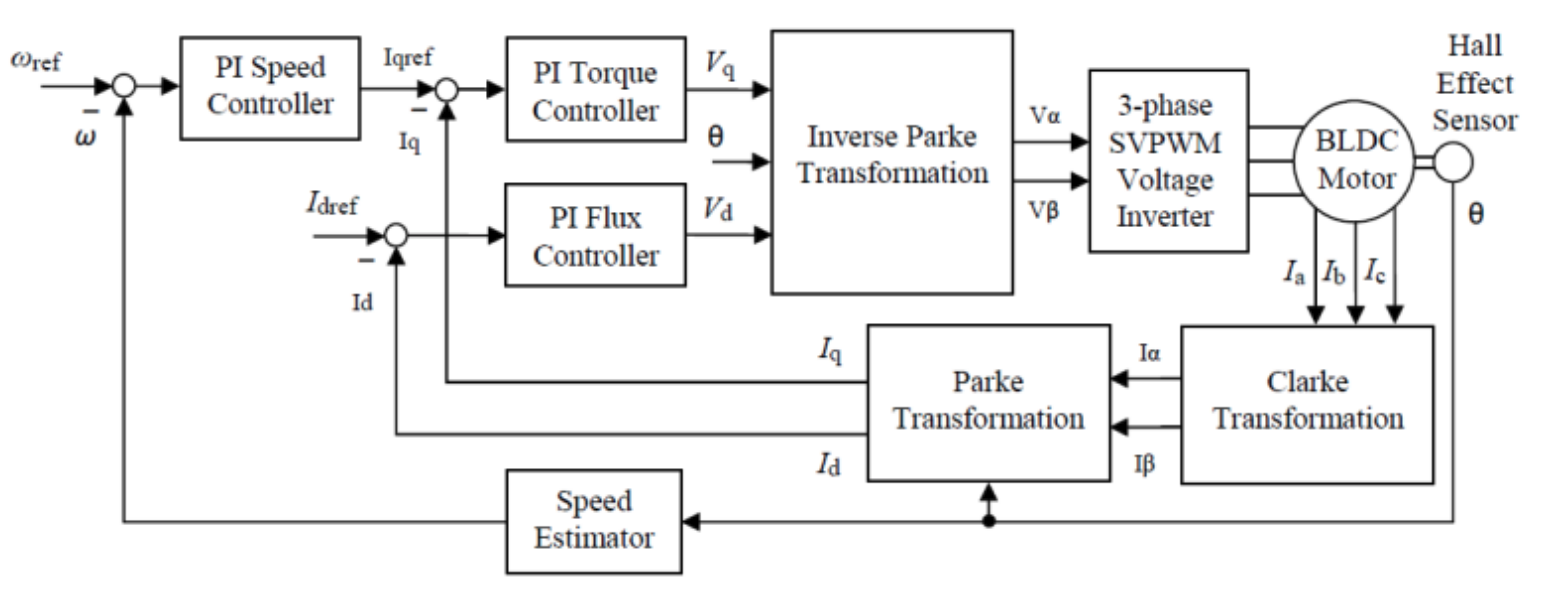
\includegraphics[width=0.95\textwidth]{figs/foc_diagram.png}
    \caption{Field Oriented Control block diagram. \cite{block_diagram_foc}}
    \label{fig:foc_diagram}
\end{figure}

The Figure~\ref{fig:foc_diagram} shows the cascaded structure of the FOC control system. 



\section{Clarke transformation}
Clarke transformation is used to transform three phase currents ($i_a$, $i_b$, $i_c$) into two orthogonal currents ($i_\alpha$, $i_\beta$) in a stationary reference frame,
where $i_\alpha$ is torque generating current and $i_\beta$ is flux producing current.

Clarke transformation can be represented as a matrix multiplication of the three phase currents with the transformation matrix
\begin{equation}
\begin{bmatrix}
i_\alpha \\
i_\beta
\end{bmatrix}
=
\frac{2}{3}
\begin{bmatrix}
1 & -\frac{1}{2} & -\frac{1}{2} \\
0 & \frac{\sqrt{3}}{2} & -\frac{\sqrt{3}}{2}
\end{bmatrix}
\begin{bmatrix}
i_a \\
i_b \\
i_c
\end{bmatrix}.
\end{equation}

The scaling factor $\frac{2}{3}$ ensures amplitude invariance between the three-phase and $i_\alpha$ $i_\beta$ representations.

The Figure~\ref{fig:clarke_transformation} shows a Clarke transformation of 3-phase sinusoidal current into two orhogonal currents. 

\begin{figure}[h]
    \centering
    \includegraphics[width=0.95\textwidth]{figs/clarke_transformation.pdf}
    \caption{Clarke transformation of three-phase current.}
    \label{fig:clarke_transformation}.
\end{figure}

% The Figure~\ref{fig:clarke_transformation} shows a Clarke transformation of 3-phase sinusoidal current. 


Inverse Clarke transformation in context of FOC is used to transform two orthogonal voltages ($v_\alpha$, $v_\beta$) in a stationary reference frame back
to three phase voltages ($v_a$, $v_b$, $v_c$) that can be applied to the stator windings and can be expressed as
\begin{equation}
\begin{bmatrix}
v_a \\
v_b \\
v_c
\end{bmatrix}
=
\begin{bmatrix}
1 & 0 \\
-\frac{1}{2} & \frac{\sqrt{3}}{2} \\
-\frac{1}{2} & -\frac{\sqrt{3}}{2}
\end{bmatrix}
\begin{bmatrix}
v_\alpha \\
v_\beta
\end{bmatrix}.
\end{equation}





\section{Park transformation}
Park transformation is used to transform two orthogonal currents ($i_\alpha$, $i_\beta$) in a stationary reference frame from the stator point of view
into two DC currents ($i_d$, $i_q$) in a rotating reference frame from a rotor point of view, where $i_d$ is a flux current and $i_q$ is a torque current.
To perfrom Park transformation, the electrical angle $\theta_e$ must to be calculated based on the rotor position, which can be obtained from the encoder reading.

Park transformation can be represented as a matrix multiplication of the two orthogonal currents ($i_\alpha$, $i_\beta$) with the transformation matrix

\begin{equation}
\begin{bmatrix}
    i_d \\
    i_q
\end{bmatrix}
=
\begin{bmatrix}
\cos(\theta_e) & \sin(\theta_e) \\
\sin(-\theta_e) & \cos(\theta_e)
\end{bmatrix}
\begin{bmatrix}
    i_\alpha \\
    i_\beta
\end{bmatrix} .
\end{equation}


Figure~\ref{fig:park_transformation} shows the Park transformation applied to the output of the 
Clarke transformation shown in Figure~\ref{fig:clarke_transformation}, resulting in two DC current components.

\begin{figure}[h]
    \centering
    \includegraphics[width=0.95\textwidth]{figs/park_transformation.pdf}
    \caption{Park transformation of Clarke transformation output}
    \label{fig:park_transformation}
\end{figure}

% The Figure~\ref{fig:park_transformation} shows Park transformation of the previous output of Clarke transformation from Figure~\ref{fig:clarke_transformation}.




In context of FOC, inverse Park transformation is used to transform two orthogonal DC voltages ($v_d$, $v_q$), which are the outputs of the PI controllers, 
from a rotating reference frame back to two orthogonal voltages ($v_\alpha$, $v_\beta$) in a stationary reference frame.

Inverse park transformation can be represented as a matrix multiplication of the two orthogonal DC voltages ($v_d$, $v_q$) with the transformation matrix
\begin{equation}
\begin{bmatrix}
v_\alpha \\
v_\beta
\end{bmatrix}
=
\begin{bmatrix}\cos(\theta_e) & -\sin(\theta_e) \\
\sin(\theta_e) & \cos(\theta_e)
\end{bmatrix}
\begin{bmatrix}v_d \\
v_q
\end{bmatrix}.
\end{equation}

\section{PI and PID regulators}

Proportional-Integral (PI) controllers are used in the FOC algorithm to regulate the $d$-axis and $q$-axis currents by adjusting the corresponding voltages ($v_d$, $v_q$).
To prevent integrator windup during saturation conditions, anti-windup protection is implemented by limiting the integration process. 
The discrete-time PI controller with anti-windup can be expressed as

\begin{equation}
x_{out}(k+1) =
K_p x_{in}(k)
+
w_{up} K_i T_s x_{in}(k)
+
x_{out}(k),
\end{equation}

where

\begin{equation}
w_{up} =
\begin{cases}
1, & \text{if } -x_{lim} < x_{in}(k) < x_{lim} \\
0, & \text{otherwise}
\end{cases}
\end{equation}

and $x_{lim}$ is the integral component limit. \cite{prayogo_foc}

The proportional term provides immediate response to the control error, while the integral term eliminates steady-state error.
In the implemented cascaded control structure, PI controllers are used for current and velocity regulation.

For position control, a Proportional-Integral-Derivative (PID) controller is additionally used to improve damping and reduce overshoot.
The PID controller generates the target angular velocity for the inner velocity control loop. \cite{SimpleFOC}


\section{Space vector modulation}

Space Vector Pulse Width Modulation (SVPWM) is used to efficiently generate three-phase PWM signals for the inverter from the calculated voltage references.
Compared to sinusoidal PWM, SVPWM provides better utilization of the DC bus voltage and allows approximately 15~\% higher maximum output voltage. \cite{svpwm_efficiency}
After inverse Park and inverse Clarke transformations generate the three-phase voltage references ($v_a$, $v_b$, $v_c$),
SVPWM computes the duty cycles for individual inverter phases and applies them to the MOSFET bridge.

The simplified SVPWM duty cycle equation can be expressed as

\begin{equation}
d_i = 0.5V_{dc} + v_{ref_i} + U^{*},
\end{equation}

where

\begin{equation}
U^{*} = -0.5 \left( \max\left(\sum_i v_{ref_i}\right) + \min\left(\sum_i v_{ref_i}\right) \right),
\end{equation}

and $v_{ref_i}$ represents the phase voltage references for phases $a$, $b$, and $c$. \cite{prayogo_foc}

\section{Velocity and position control loops}

The FOC torque control loop directly regulates the motor torque through the $i_q$ current component.
Once torque control is established, higher-level control loops can be added on top of the inner current loop in order to control additional mechanical quantities.

Angular velocity control can implemented using a cascaded control structure. \cite{SimpleFOC}
The measured motor velocity derived from encoder readings is compared with the target velocity, 
and the resulting error is processed by a PI controller.
The output of the velocity controller generates the target torque-producing current $i_q$ for the inner FOC current control loop.
In this way, motor velocity is indirectly controlled through regulation of the generated motor torque.

Similarly, position control can be implemented as an additional outer control loop.
The measured rotor position is compared with the target position, and the resulting position error is processed by a PID controller.
The output of the position controller generates the target angular velocity for the velocity control loop.

This creates a cascaded control hierarchy consisting of:
\begin{itemize}
    \item current control loop regulating motor torque,
    \item velocity control loop regulating angular velocity,
    \item position control loop regulating rotor position.
\end{itemize}

The cascaded structure allows simultaneous control of motor torque, angular velocity, and position while maintaining stable dynamic behaviour.
Typically, the inner current loop operates at the highest update frequency, while the outer velocity and position loops operate at lower frequencies
due to slower mechanical system dynamics.

\section{Electrical angle calculation}

